\documentclass[12pt,a4paper,fleqn]{article}
\usepackage[utf8]{inputenc}
\usepackage[russian]{babel}
\usepackage{amssymb, amsmath, multicol}
\usepackage{enumitem}
\usepackage{lipsum}
\usepackage{euler}
\oddsidemargin=-15.4mm
\textwidth=190mm
\headheight=-32.4mm
\textheight=277mm
\parindent=0pt
\parskip=8pt
\pagestyle{empty}
\usepackage{graphicx}
\title{\textbf{\LARGE{Исследовательская работа по теме:\\Исследование функции дифференциальными методами}}}
\author{Известный гражданин}
\date{November 2022}
\addt\captionsrussian{\def\refname{Список литературы}}\begin{document}
\maketitle
\newpage\newpage \textbf{\LARGE{Глава I. Функция}}

\begin{center}
$y = $$(sin(x)+cos(x)) \cdot 2$

\end{center}
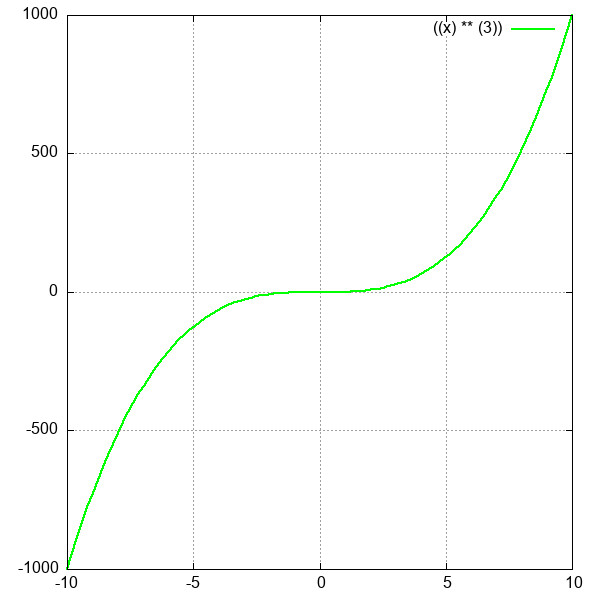
\includegraphics{GraphicDumps/plot.jpg}\newpage \textbf{\LARGE{Глава II. Визуальный анализ функции}}

Говорят

\begin{center}
$y = $$(sin(x)+cos(x)) \cdot 2$

\end{center}
\newpage \textbf{\LARGE{Глава III. Дифференцирование}}

Поэтому

\begin{center}
 ($x)'
  = 1$\end{center}
Вычислительные ошибки уйдут, достаточно просто...

\begin{center}
 ($sin(x))'
  = 1 \cdot cos(x)$\end{center}
Продвинутый читатель уже заметил, что

\begin{center}
 ($x)'
  = 1$\end{center}
(null)\cite{link4}

\begin{center}
 ($cos(x))'
  = 1 \cdot (0-sin(x))$\end{center}
//TODO: Лёша, придумай переход. У меня идеи закончились

\begin{center}
 ($sin(x)+cos(x))'
  = 1 \cdot cos(x)+1 \cdot (0-sin(x))$\end{center}
\\ title{не сложно заметить} 

\begin{center}
 ($2)'
  = 0$\end{center}
Вы не шокированы?\cite{link3}

\begin{center}
 ($(sin(x)+cos(x)) \cdot 2)'
  = (1 \cdot cos(x)+1 \cdot (0-sin(x))) \cdot 2+(sin(x)+cos(x)) \cdot 0$\end{center}
\newpage \textbf{\LARGE{Глава IV.Упрощение выражения}}

Отметим, что

\begin{center}
$1 \cdot cos(x) = cos(x)$\end{center}
Ну вот как этот матан тебе в жизни пригодится?

\begin{center}
$1 \cdot (0-sin(x)) = 0-sin(x)$\end{center}
Говорят

\begin{center}
$(sin(x)+cos(x)) \cdot 0 = 0$\end{center}
По теореме Эскобара

\begin{center}
$(cos(x)+(0-sin(x))) \cdot 2+0 = (cos(x)+(0-sin(x))) \cdot 2$\end{center}
\newpage \textbf{\LARGE{Глава V. Полученая производная}}

$y = $$(sin(x)+cos(x)) \cdot 2$

$y' = $$(cos(x)+(0-sin(x))) \cdot 2$

\includegraphics{GraphicDumps/plot_1.jpg}\newpage \textbf{\LARGE{Глава VI. Разложение функции по формуле Тейлора}}

Единственное, что я не понимаю, так это то, зачем ты это читаешь

\begin{center}
\end{center}
\begin{center}$sin(0) = 0$\end{center}
Господи, да для кого я вообще стараюсь

\begin{center}
\end{center}
\begin{center}$cos(0) = 1$\end{center}
Откуда

\begin{center}
\end{center}
\begin{center}$0+1 = 1$\end{center}
А теперь уберите детей от экранов

\begin{center}
\end{center}
\begin{center}$1 \cdot 2 = 2$\end{center}
Телец в козероге, поэтому

\begin{center}
 ($x)'
  = 1$\end{center}
Говорят

\begin{center}
 ($sin(x))'
  = 1 \cdot cos(x)$\end{center}
Доказательство данного факта предоставлено лицом или организацией исполняющей функции иностанного агента

\begin{center}
 ($x)'
  = 1$\end{center}
Продвинутый читатель уже заметил, что

\begin{center}
 ($cos(x))'
  = 1 \cdot (0-sin(x))$\end{center}
Таким образом

\begin{center}
 ($sin(x)+cos(x))'
  = 1 \cdot cos(x)+1 \cdot (0-sin(x))$\end{center}
//TODO: Лёша, придумай переход. У меня идеи закончились

\begin{center}
 ($2)'
  = 0$\end{center}
Не так страшна производная, как её находят\cite{link2}

\begin{center}
 ($(sin(x)+cos(x)) \cdot 2)'
  = (1 \cdot cos(x)+1 \cdot (0-sin(x))) \cdot 2+(sin(x)+cos(x)) \cdot 0$\end{center}
Ну ты же всё равно не будешь это проверять

\begin{center}
$1 \cdot cos(x) = cos(x)$\end{center}
Здесь могла быть ваша реклама

\begin{center}
$1 \cdot (0-sin(x)) = 0-sin(x)$\end{center}
Доказательство данного факта предоставлено лицом или организацией исполняющей функции иностанного агента

\begin{center}
$(sin(x)+cos(x)) \cdot 0 = 0$\end{center}
Нам не объяснили на семинаре как это делать, поэтому примем на веру

\begin{center}
$(cos(x)+(0-sin(x))) \cdot 2+0 = (cos(x)+(0-sin(x))) \cdot 2$\end{center}
Дифференциал Елена всего в 100 метрах от вас...

\begin{center}
\end{center}
\begin{center}$cos(0) = 1$\end{center}
Если посмотреть на выражение под другим углом, можно получить

\begin{center}
\end{center}
\begin{center}$sin(0) = 0$\end{center}
Ты же продолжаешь читать, да?

\begin{center}
\end{center}
\begin{center}$0-0 = 0$\end{center}
Нам не объяснили на семинаре как это делать, поэтому примем на веру

\begin{center}
\end{center}
\begin{center}$1+0 = 1$\end{center}
Без комментариев\cite{link4}

\begin{center}
\end{center}
\begin{center}$1 \cdot 2 = 2$\end{center}
Руководствуясь сборником <<Задачи для подготовки к поступлению в советские ясли>>\cite{link1}

\begin{center}
\end{center}
\begin{center}$\frac{2}{1} = 2$\end{center}
При этом

\begin{center}
$x-0 = x$\end{center}
Кроме того

\begin{center}
$x^{1} = x$\end{center}
Если вы понимаете данный переход, то я вам сочувствую

\begin{center}
 ($x)'
  = 1$\end{center}
//TODO: Лёша, придумай переход. У меня идеи закончились

\begin{center}
 ($cos(x))'
  = 1 \cdot (0-sin(x))$\end{center}
Паршивая функция всё доказательство портит\cite{link2}

\begin{center}
 ($0)'
  = 0$\end{center}
Отметим, что

\begin{center}
 ($x)'
  = 1$\end{center}
Вычислительные ошибки уйдут, достаточно просто...

\begin{center}
 ($sin(x))'
  = 1 \cdot cos(x)$\end{center}
Продвинутый читатель уже заметил, что

\begin{center}
 ($0-sin(x))'
  = 0-1 \cdot cos(x)$\end{center}
[Данные удалены]

\begin{center}
 ($cos(x)+(0-sin(x)))'
  = 1 \cdot (0-sin(x))+(0-1 \cdot cos(x))$\end{center}
Дифференциал - серебро, производная золото\cite{link2}

\begin{center}
 ($2)'
  = 0$\end{center}
Телец в козероге, поэтому

\begin{center}
A = $(1 \cdot (0-sin(x))+(0-1 \cdot cos(x))) \cdot 2$\end{center}
\begin{center}
 ($(cos(x)+(0-sin(x))) \cdot 2)'
  = A+(cos(x)+(0-sin(x))) \cdot 0$\end{center}
Используя выводы из теоремы 1000-7 получаем

\begin{center}
$1 \cdot (0-sin(x)) = 0-sin(x)$\end{center}
Кроме того

\begin{center}
$1 \cdot cos(x) = cos(x)$\end{center}
Поэтому

\begin{center}
$(cos(x)+(0-sin(x))) \cdot 0 = 0$\end{center}
Руководствуясь базовой логикой, получаем

\begin{center}
$((0-sin(x))+(0-cos(x))) \cdot 2+0 = ((0-sin(x))+(0-cos(x))) \cdot 2$\end{center}
Вычислительные ошибки уйдут, достаточно просто...

\begin{center}
\end{center}
\begin{center}$sin(0) = 0$\end{center}
Без комментариев\cite{link4}

\begin{center}
\end{center}
\begin{center}$0-0 = 0$\end{center}
Любовь - это верить в его выводы без доказательств...

\begin{center}
\end{center}
\begin{center}$cos(0) = 1$\end{center}
Доказательство данного факта предоставлено лицом или организацией исполняющей функции иностанного агента

\begin{center}
\end{center}
\begin{center}$0-1 = -1$\end{center}
Segmentation fault (core dumped)

\begin{center}
\end{center}
\begin{center}$0+-1 = -1$\end{center}
Функция производной не стоит\cite{link2}

\begin{center}
\end{center}
\begin{center}$-1 \cdot 2 = -2$\end{center}
Паршивая функция всё доказательство портит\cite{link2}

\begin{center}
\end{center}
\begin{center}$\frac{-2}{2} = -1$\end{center}
Обоснование этого пререхода предостовляется читателю в качестве несложного упрожнения

\begin{center}
$x-0 = x$\end{center}
Дифференциал Елена всего в 100 метрах от вас...

\begin{center}
 ($0)'
  = 0$\end{center}
Единственное, что я не понимаю, так это то, зачем ты это читаешь

\begin{center}
 ($x)'
  = 1$\end{center}
Только 0.00001 процент умнейших людей планеты смогут понять этот переход

\begin{center}
 ($sin(x))'
  = 1 \cdot cos(x)$\end{center}
По теореме Эскобара

\begin{center}
 ($0-sin(x))'
  = 0-1 \cdot cos(x)$\end{center}
(null)\cite{link4}

\begin{center}
 ($0)'
  = 0$\end{center}
Если посмотреть на выражение под другим углом, можно получить

\begin{center}
 ($x)'
  = 1$\end{center}
Оказывается

\begin{center}
 ($cos(x))'
  = 1 \cdot (0-sin(x))$\end{center}
[Данные удалены]

\begin{center}
 ($0-cos(x))'
  = 0-1 \cdot (0-sin(x))$\end{center}
Используя выводы из теоремы 1000-7 получаем

\begin{center}
 ($(0-sin(x))+(0-cos(x)))'
  = (0-1 \cdot cos(x))+(0-1 \cdot (0-sin(x)))$\end{center}
Кроме того

\begin{center}
 ($2)'
  = 0$\end{center}
По теореме Эскобара

\begin{center}
A = $(0-1 \cdot cos(x))+(0-1 \cdot (0-sin(x)))$\end{center}
\begin{center}
 ($((0-sin(x))+(0-cos(x))) \cdot 2)'
  = (A) \cdot 2+((0-sin(x))+(0-cos(x))) \cdot 0$\end{center}
Вы не шокированы?\cite{link3}

\begin{center}
$1 \cdot cos(x) = cos(x)$\end{center}
Отметим, что

\begin{center}
$1 \cdot (0-sin(x)) = 0-sin(x)$\end{center}
Ребята не стоит разбираться в этом переходе. Вы молодые, шутливые, вам все легко. Это не то. Это не Чикатило и даже не архивы спецслужб. Сюда лучше не лезть. Серьезно, любой из вас будет жалеть. Лучше закройте тему и забудьте что тут писалось. Я вполне понимаю что данным сообщением вызову дополнительный интерес, но хочу сразу предостеречь пытливых - стоп. Остальных просто не найдут.

\begin{center}
$((0-sin(x))+(0-cos(x))) \cdot 0 = 0$\end{center}
Если вы не понимаете этот переход, то я вам сочувствую

\begin{center}
$((0-cos(x))+(0-(0-sin(x)))) \cdot 2+0 = ((0-cos(x))+(0-(0-sin(x)))) \cdot 2$\end{center}
Хорошо там, где производной нет\cite{link2}

\begin{center}
\end{center}
\begin{center}$cos(0) = 1$\end{center}
Продвинутый читатель уже заметил, что

\begin{center}
\end{center}
\begin{center}$0-1 = -1$\end{center}
Ну вот как этот матан тебе в жизни пригодится?

\begin{center}
\end{center}
\begin{center}$sin(0) = 0$\end{center}
Кроме того

\begin{center}
\end{center}
\begin{center}$0-0 = 0$\end{center}
Отметим, что

\begin{center}
\end{center}
\begin{center}$0-0 = 0$\end{center}
Очевидно, что

\begin{center}
\end{center}
\begin{center}$-1+0 = -1$\end{center}
Не трудно заметить

\begin{center}
\end{center}
\begin{center}$-1 \cdot 2 = -2$\end{center}
Если вы понимаете данный переход, то я вам сочувствую

\begin{center}
\end{center}
\begin{center}$\frac{-2}{6} = -0.333333$\end{center}
Господи, да для кого я вообще стараюсь

\begin{center}
$x-0 = x$\end{center}
Segmentation fault (core dumped)

\begin{center}
 ($0)'
  = 0$\end{center}
Нам не объяснили на семинаре как это делать, поэтому примем на веру

\begin{center}
 ($x)'
  = 1$\end{center}
Хорошо там, где производной нет\cite{link2}

\begin{center}
 ($cos(x))'
  = 1 \cdot (0-sin(x))$\end{center}
По теореме Эскобара

\begin{center}
 ($0-cos(x))'
  = 0-1 \cdot (0-sin(x))$\end{center}
Оказывается

\begin{center}
 ($0)'
  = 0$\end{center}
Руководствуясь базовой логикой, получаем

\begin{center}
 ($0)'
  = 0$\end{center}
Вычислительные ошибки уйдут, достаточно просто...

\begin{center}
 ($x)'
  = 1$\end{center}
По лемме $\sqrt{-759}$
\begin{center}
 ($sin(x))'
  = 1 \cdot cos(x)$\end{center}
Поэтому

\begin{center}
 ($0-sin(x))'
  = 0-1 \cdot cos(x)$\end{center}
По теореме Эскобара

\begin{center}
 ($0-(0-sin(x)))'
  = 0-(0-1 \cdot cos(x))$\end{center}
Для любого эпсилон больше нулю очевидно, что

\begin{center}
 ($(0-cos(x))+(0-(0-sin(x))))'
  = (0-1 \cdot (0-sin(x)))+(0-(0-1 \cdot cos(x)))$\end{center}
//TODO: Лёша, придумай переход. У меня идеи закончились

\begin{center}
 ($2)'
  = 0$\end{center}
Хорошо там, где производной нет\cite{link2}

\begin{center}
A = $(0-1 \cdot (0-sin(x)))+(0-(0-1 \cdot cos(x)))$\end{center}
\begin{center}
 ($((0-cos(x))+(0-(0-sin(x)))) \cdot 2)'
  = (A) \cdot 2+((0-cos(x))+(0-(0-sin(x)))) \cdot 0$\end{center}
Если посмотреть на выражение под другим углом, можно получить

\begin{center}
$1 \cdot (0-sin(x)) = 0-sin(x)$\end{center}
Здесь могла быть ваша реклама

\begin{center}
$1 \cdot cos(x) = cos(x)$\end{center}
Руководствуясь базовой логикой, получаем

\begin{center}
$((0-cos(x))+(0-(0-sin(x)))) \cdot 0 = 0$\end{center}
Господи, да для кого я вообще стараюсь

\begin{center}
A = $((0-(0-sin(x)))+(0-(0-cos(x)))) \cdot 2$\end{center}
\begin{center}
$A+0 = ((0-(0-sin(x)))+(0-(0-cos(x)))) \cdot 2$\end{center}
Господи, да для кого я вообще стараюсь

\begin{center}
\end{center}
\begin{center}$sin(0) = 0$\end{center}
Говорят

\begin{center}
\end{center}
\begin{center}$0-0 = 0$\end{center}
В ближайшее время ожидаются осадки из ваших слёз от попыток понять этот переход

\begin{center}
\end{center}
\begin{center}$0-0 = 0$\end{center}
Доказательство данного факта предоставлено лицом или организацией исполняющей функции иностанного агента

\begin{center}
\end{center}
\begin{center}$cos(0) = 1$\end{center}
Паршивая функция всё доказательство портит\cite{link2}

\begin{center}
\end{center}
\begin{center}$0-1 = -1$\end{center}
Положим

\begin{center}
\end{center}
\begin{center}$0--1 = 1$\end{center}
Для любого эпсилон больше нулю очевидно, что

\begin{center}
\end{center}
\begin{center}$0+1 = 1$\end{center}
Нам не объяснили на семинаре как это делать, поэтому примем на веру

\begin{center}
\end{center}
\begin{center}$1 \cdot 2 = 2$\end{center}
А теперь уберите детей от экранов

\begin{center}
\end{center}
\begin{center}$\frac{2}{24} = 0.0833333$\end{center}
Обоснование этого пререхода предостовляется читателю в платном DLC

\begin{center}
$x-0 = x$\end{center}
Только 0.00001 процент умнейших людей планеты смогут понять этот переход

\begin{center}
 ($0)'
  = 0$\end{center}
Если вы понимаете данный переход, то я вам сочувствую

\begin{center}
 ($0)'
  = 0$\end{center}
Говорят

\begin{center}
 ($x)'
  = 1$\end{center}
Господи, да для кого я вообще стараюсь

\begin{center}
 ($sin(x))'
  = 1 \cdot cos(x)$\end{center}
Ну ты же всё равно не будешь это проверять

\begin{center}
 ($0-sin(x))'
  = 0-1 \cdot cos(x)$\end{center}
Не трудно заметить

\begin{center}
 ($0-(0-sin(x)))'
  = 0-(0-1 \cdot cos(x))$\end{center}
Если вы не понимаете этот переход, то я вам сочувствую

\begin{center}
 ($0)'
  = 0$\end{center}
[Данные удалены]

\begin{center}
 ($0)'
  = 0$\end{center}
Если вы понимаете данный переход, то я вам сочувствую

\begin{center}
 ($x)'
  = 1$\end{center}
Я придумал поистине удивительное доказательство этого факта, но поля этой книги слишком малы\ldots

\begin{center}
 ($cos(x))'
  = 1 \cdot (0-sin(x))$\end{center}
Господи, да для кого я вообще стараюсь

\begin{center}
 ($0-cos(x))'
  = 0-1 \cdot (0-sin(x))$\end{center}
Хорошо там, где производной нет\cite{link2}

\begin{center}
 ($0-(0-cos(x)))'
  = 0-(0-1 \cdot (0-sin(x)))$\end{center}
Руководствуясь базовой логикой, получаем

\begin{center}
 ($(0-(0-sin(x)))+(0-(0-cos(x))))'
  = (0-(0-1 \cdot cos(x)))+(0-(0-1 \cdot (0-sin(x))))$\end{center}
Имеем

\begin{center}
 ($2)'
  = 0$\end{center}
Дефии... кхм, Дифири... тьфу ты, дифферин... Да что ж со мной такое сегодня? Дифференциал. Уф, совсем я заработался. Пойду отдохну *звук отодвигаемого стула, затем удаляющихся шагов*

\begin{center}
A = $(0-(0-1 \cdot cos(x)))+(0-(0-1 \cdot (0-sin(x))))$\end{center}
\begin{center}
B = $((0-(0-sin(x)))+(0-(0-cos(x)))) \cdot 0$\end{center}
\begin{center}
 ($((0-(0-sin(x)))+(0-(0-cos(x)))) \cdot 2)'
  = (A) \cdot 2+B$\end{center}
Руководствуясь сборником <<Задачи для подготовки к поступлению в советские ясли>>\cite{link1}

\begin{center}
$1 \cdot cos(x) = cos(x)$\end{center}
Спешка нужна только в армии и при ловле блох. Но не как уж ни при вычислении производной\cite{link2}

\begin{center}
$1 \cdot (0-sin(x)) = 0-sin(x)$\end{center}
Здесь могла быть ваша реклама

\begin{center}
$((0-(0-sin(x)))+(0-(0-cos(x)))) \cdot 0 = 0$\end{center}
Кроме того

\begin{center}
A = $(0-(0-cos(x)))+(0-(0-(0-sin(x))))$\end{center}
\begin{center}
$(A) \cdot 2+0 = (A) \cdot 2$\end{center}
Оказывается

\begin{center}
\end{center}
\begin{center}$cos(0) = 1$\end{center}
Автору приснилось, что следующее преобразование верно

\begin{center}
\end{center}
\begin{center}$0-1 = -1$\end{center}
Ну ты же всё равно не будешь это проверять

\begin{center}
\end{center}
\begin{center}$0--1 = 1$\end{center}
Дураку понятно, что

\begin{center}
\end{center}
\begin{center}$sin(0) = 0$\end{center}
Дифференциал - серебро, производная золото\cite{link2}

\begin{center}
\end{center}
\begin{center}$0-0 = 0$\end{center}
Для любого эпсилон больше нулю очевидно, что

\begin{center}
\end{center}
\begin{center}$0-0 = 0$\end{center}
По теореме Эскобара

\begin{center}
\end{center}
\begin{center}$0-0 = 0$\end{center}
Я придумал поистине удивительное доказательство этого факта, но поля этой книги слишком малы\ldots

\begin{center}
\end{center}
\begin{center}$1+0 = 1$\end{center}
(null)\cite{link4}

\begin{center}
\end{center}
\begin{center}$1 \cdot 2 = 2$\end{center}
Кроме того

\begin{center}
\end{center}
\begin{center}$\frac{2}{120} = 0.0166667$\end{center}
Ну ты же всё равно не будешь это проверять

\begin{center}
$x-0 = x$\end{center}
\textbf{\LARGE{Получим разложение по формуле Тейлора:}}
\begin{center}
$y = $$2+(2 \cdot x+(-1 \cdot x^{2}+(-0.333333 \cdot x^{3}+(0.0833333 \cdot x^{4}+0.0166667 \cdot x^{5}))))$$ + o(x^{5})$
\end{center}
\newpage\begin{thebibliography}{}
\bibitem{link1}  "A Synopsis of Elementary Results in Pure and Applied Mathematics"
\bibitem{link2}  "Сборник пословиц и поговорок кафедры высшей математики"
\bibitem{link3}  "Полное собрание лучших высказываний преподавателей МФТИ"
\bibitem{link4}  "Словарь фраз не несущих смысловой нагрузки кафедры философии. 17 издание"
\end{thebibliography}\end{document}